\section{Robustness}
As said previously, the "critical" operations are the primitive geometric operations as they determine the correctness of the code. Even if the questions of "in/out circle" and "left/right segment" might seem obvious, the problems of floating numbers which can occur are sensitive issues. In this section, we present why these problems arise and how they are handled.

One may define (\cite{schirra}) the robustness as the ability of an algorithm to produce the correct result for some perturbation of the input. As we will see, rounding errors in floating point arithmetic are such perturbations.

\subsection{Floating number}
We first have a look at how does the computer store and handle problems. As a computer does not have infinite precision, the real numbers are stored in the computer as \textit{floating numbers} (\cite{VLegat},\cite{schirra}). A floating number has a base $B$, a fixed mantissa length $l$ and an exponent $e$ : 
\begin{equation*}
± \underbrace{d_0.d_1 d_2 \cdots d_{l-1}}_l * B^e.
\end{equation*}
It is \textit{normalized} if $d_0=0$. As numbers are represented as finite floating point, rounding error may occur. This lead to numerical error. Let $a$ be a number and $a_f$ its floating number representation. We define the \textit{absolute error} as $|a-a_f|$ and the \textit{relative error} as $|a-a_f|/|a|$. The relative error is bounded by the \textit{machine epsilon}, this is $\frac{B}{2} B^{-l}$. The way the machine makes the rounding operation is defined by the IEEE standard 754.

These floating numbers can be stored in \textit{simple precision} (32 bit word, this is $e\in [-126,127]$; \texttt{float} in C) or \textit{double precision} (64 bit word, this is $e\in [-1022,1023]$ and $l=53$; \texttt{double} in C).

Let's give an example of the dramatic effect these rounding might involve. Let define three number $a=5.6543723$, $b=5.654371$ and $c=0.000001$ and their floating number representation if mantissa length is $l=6$ : $a_f=0.565437 \cdot 10^1$, $b_f=0.565437 \cdot 10^1$ and $c=0.1 \cdot 10^{-5}$. we have : 
\begin{align*}
a-b-c &= 3 \cdot 10^{-07} \\
a_f - b_f - c_f &= - 0.1 \cdot 10^{-5}
\end{align*} 
Where these two simple expression does not even have the same sign!

\subsection{Primitive geometric operations and determinant}
In numerical geometry, many primitive operations (as the inclusion in a circle or the orientation problem) consist of evaluating the sign of a determinant (\cite{bronnimann2000efficient}, \cite{robust}).

Let $\overrightarrow{ab}$ be an oriented segment and $c$ a point. Determine whether $c$ lies on the left or on the right of $\overrightarrow{ab}$ can be solve by evaluating the sign of the following determinant : 
\begin{align}
& \det \begin{pmatrix}
a_x & a_y & 1\\
b_x & b_y & 1\\
c_x & c_y & 1
\end{pmatrix} \label{eq:detOrientation1}\\
\Leftrightarrow & \det \begin{pmatrix}
a_x - c_x & a_y - c_y \\
b_x - c_x & b_y - c_y
\end{pmatrix} \label{eq:detOrientation2}
\end{align}
if this determinant is positive, $c$ lies on the right of $\overrightarrow{ab}$, if negative, on the left and if null, on the segment.


Now let $abc$ be an oriented circle (meaning that $a$, $b$ and $c$ are points on the circle, occurring in counter-clockwise order), and $d$ a point. Determine whether $d$ lies inside or outside the circle $abc$ can be solve by evaluating the sign of the following determinant : 
\begin{align}
& \det \begin{pmatrix}
a_x & a_y & a_x^2 + a_y ^2 & 1\\
b_x & b_y & b_x^2 + b_y^2 & 1\\
c_x & c_y & c_x^2+c_y^2 & 1 \\
d_x & d_y & d_x^2+d_y^2 & 1
\end{pmatrix} \label{eq:Incircle1}\\
\Leftrightarrow & \det \begin{pmatrix}
a_x-d_x & a_y-d_y & (a_x-d_x)^2 + (a_y - d_y)^2\\
b_x-d_x & b_y - d_y & (b_x-d_x)^2 + (b_y - d_y)^2\\
c_x-d_x & c_y - d_y & (c_x-d_x)^2 + (c_y - d_y)^2
\end{pmatrix} \label{eq:Incircle2}
\end{align}
If the determinant is positive, $d$ lies inside the circle, if negative, outside and if null, on the circle.

So we see that these primitive operation correspond to evaluate the sign of a determinant. As explained previously, in floating point representation, rounding error may occur. And as we have seen in an example, this might even change the sign of an expression. So evaluate these determinant is a critical issue.

A first idea to reduce the numerical error is to compute it in a numerical "robust" way. The determinant above are already a "not so bad" way to make these geometric tests (we might have build more "hard-coded" manner less robust). Moreover, it turns out (\cite{shewchuk1996robust}) that formulation \eqref{eq:detOrientation2} and\eqref{eq:Incircle2} are better in terms of error propagation that \eqref{eq:Incircle1} and \eqref{eq:detOrientation1}.
So this are the first "non-robust" (but acceptable) methods that we implemented in our functions \texttt{leftRightSegment} and \texttt{isInsideGen} (if they are called with \texttt{ROBUST=0}).

But these method remains non-robust and are not design to resist to extreme cases. This are cases where the evaluation of the sign of the determinant might fail. The next sections introduce methods to deal with these issues. Notice that the fact that these methods are non-robust does not mean that they are bad. Indeed the limit cases we are handling now occurs a very few times so the non-robust method work well most of the time. 

\subsection{Magic epsilon}
A very common idea (\cite{schirra}) would be to use a bound saying "\textit{if something is closed to zero, it is zero}". This is, setting a $\epsilon _{magic}$ and say if $a-b<\epsilon _{magic} \Rightarrow a=b$. This might solve some problems and work in a lot of cases. But this approach might fail in some extreme cases and moreover, under this $\epsilon_{magic}$, the equality is not transitive. So we drop this idea.
  
\subsection{Clarkson's method}
We do not spend much time on this method as we did not implement it; we just briefly quote it for our most interested and zealous readers.\\
The idea of Clarkson's method, developed in \cite{bronnimann2000efficient}, is to evaluate the sign of the determinant of $A$, using a wise preconditioning matrix which reduce the numerical errors. Clarckson's preconditioning applies a variant of Gram-Schmidt reduction which is why it is sometimes called reorthogonalization method.


\subsection{Exact arithmetic}
A promising idea (\cite{bronnimann2000efficient}, \cite{schirra}, \cite{shewchuk1996robust}) would be to work with exact numbers, this is \textit{exact arithmetic} defined (\cite{exactArithmetic}) as : \\
\textit{In computer science, arbitrary-precision arithmetic [...] indicates that calculations are performed on numbers whose digits of precision are limited only by the available memory of the host system. This contrasts with the faster fixed-precision arithmetic [...] which typically offers between 8 and 64 bits of precision.}


For instance, exact arithmetic with \textit{rational} numbers can be done by storing two integer numbers (the numerator and denominator). Exact arithmetic for \textit{real} numbers is a little more intricate. 
On way to figure out how exact arithmetic works is to think of an arithmetic expression as an \textit{expression tree} (\cite{schirra}): the leaves are numbers and the internal nodes are operations $+,*,-,/$. \\
Arbitrary precision values are expressed as $x=x_n + \cdots + x_2 + x_1$ (where $x_i > x_{i-1}$). We call $\oplus$, $\ominus$ and $\otimes$ the $p$-bit floating point addition, subtraction and multiplication with exact rounding.
For instance, the orientation problem described above can be expressed as in figure \ref{fig:ExactArithmetic}.\\

Obviously exact arithmetic uses more memory than classical floating point arithmetic. It is also slower (significantly slower).\\

Libraries in C++ implement such exact arithmetic; for instance LEDA or LD (Fortune and Van Wyk).

\begin{figure}
  \centering
  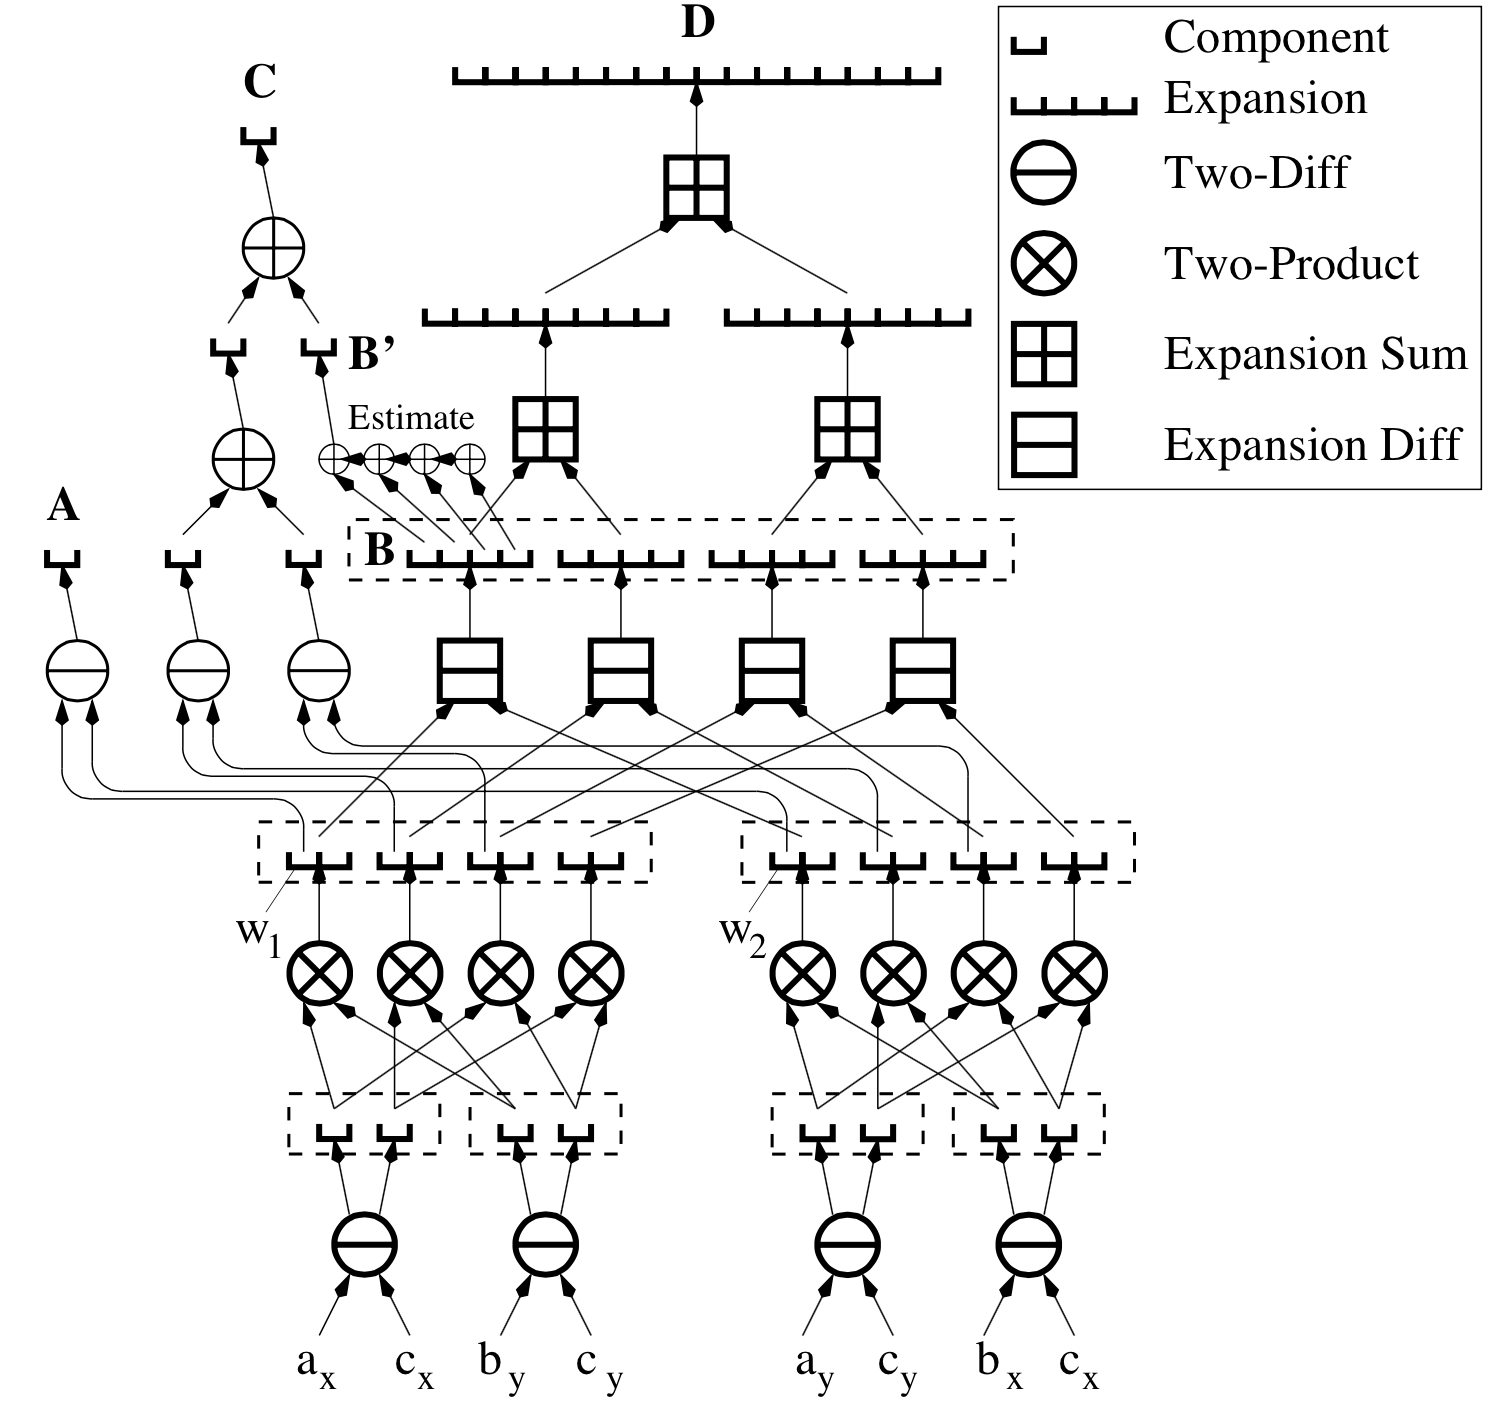
\includegraphics[width=0.5\textwidth]{images/orientation2d.png}
  \caption{Adaptive calculations used by the 2D orientation test \cite{shewchuk1996robust}.}
  \label{fig:ExactArithmetic}
\end{figure}

\subsection{Arithmetic filters}
The main inconvenient of exact arithmetic is that it is significantly slower than classical floating point arithmetic. Furthermore, we only need to use exact arithmetic for some "limit" cases. An obvious idea would be to use exact arithmetic only in some critical situations. The implementation of this method is called \textit{arithmetic filters} (\cite{schirra}, \cite{shewchuk1996robust}). The idea of floating point filters is : 
\begin{itemize}
\item compute the expression using classical floating numbers arithmetic;
\item compute a bound of the error of the floating point computation and compare it with the absolute value of the expression computed before.
\item if the error is smaller than the "exact value" of the expression and its approximation in floating point have the same sign, our approximation is acceptable;
\item if the error is bigger we have no guarantee that the sign of the floating point approximation and the exact value is the same. In this case, we use exact arithmetic computation to re-evaluate the expression.
\end{itemize}

Fortune and Van Wyk implemented such arithmetic filter.

\subsection{Implementation}
In our code, we use an implementation developed by J. R. Shewchuk (\cite{shewchuk1996robust} for the paper, \cite{robust} for the code) available in open source (downloaded in the file \texttt{robustFunctions.c}). He implemented methods using exact computation and arithmetic filters (slightly improved using computations of increasingly accuracy, cf. results $A$, $B$, $C$ or $D$ of figure \ref{fig:ExactArithmetic}, and many other heuristics...). In our functions \texttt{isInsideGen} and \texttt{leftRightSegment} we either make our non-robust implementation (if the input variable \texttt{ROBUST=0}) or we call the robust Shewchuk's functions \texttt{incircle} and \texttt{orient2d} (if the input variable \texttt{ROBUST=1}).








